% ****** Start of file apssamp.tex ******
%
%   This file is part of the APS files in the REVTeX 4.1 distribution.
%   Version 4.1r of REVTeX, August 2010
%
%   Copyright (c) 2009, 2010 The American Physical Society.
%
%   See the REVTeX 4 README file for restrictions and more information.
%
% TeX'ing this file requires that you have AMS-LaTeX 2.0 installed
% as well as the rest of the prerequisites for REVTeX 4.1
%
% See the REVTeX 4 README file
% It also requires running BibTeX. The commands are as follows:
%
%  1)  latex apssamp.tex
%  2)  bibtex apssamp
%  3)  latex apssamp.tex
%  4)  latex apssamp.tex

\documentclass[aps, pre, twocolumn, nofootinbib]{revtex4-1}

\usepackage{graphicx}% Include figure files
\usepackage{dcolumn}% Align table columns on decimal point
\usepackage{bm}% bold math
\usepackage{multirow,caption}
%\usepackage{multicols}
\usepackage{amsmath}
\usepackage{hhline}
\usepackage{color}
\usepackage{xcolor}
\usepackage[normalem]{ulem}
%\usepackage[table]{xcolor}
%\graphicspath{ {figures/} }
\usepackage{array}
\usepackage{caption}
\usepackage{subcaption}
\usepackage[thinlines]{easytable}

\setlength{\arrayrulewidth}{0.3mm}
%\setlength{\tabcolsep}{10pt}
%\renewcommand{\arraystretch}{2.5}

\begin{document}
%\stepcounter{section}
\preprint{APS/123-QED}

\title{Exploring and understanding the Interdependence of Collaboration Networks}

\author{Chakresh Kr. Singh}
\email{chakresh.singh@iitgn.ac.in}
%\affiliation{Indian Institute of Technology, Gandhinagar, India-382355}
\author{Demival Vasques Filho}
\email{d.vasques@auckland.ac.nz}
%\affiliation{University of Auckland, New Zealand}
\author{Dion O' Neale}
\email{d.oneale@auckland.ac.nz}
%\affiliation{University of Auckland, New Zealand}

\author{Shivakumar Jolad}
\email{shiva.jolad@iitgn.ac.in}
%\affiliation{University of Auckland, New Zealand}


\date{\today}

\begin{abstract}
In this project we explore the interdependence between collaboration networks (citation and co-authorship in our case). Empirical study gives us evidence of strong correlation between the growth of a citation network and its corresponding co-authorship network. Literature review suggests that the strong correlation is indicative of interdependence between the simultaneous growth of these networks and that growth of one is effected by another. Through this project we try to understand this correlation and see if it has any mathematical structure.
%\begin{description}
%\item[Keywords]

%\item[PACS numbers]
%87.19.X-, 87.10.Mn , 87.23.Ge, 05.45.Tp, 07.05.Tp
%\end{description}

\end{abstract}

%\pacs{Valid PACS appear here}
\maketitle


\section{Introduction}

Easier access to meta-data of published articles has opened up opportunities to understand the mechanism of growth of a subject and diffusion of knowledge between researchers. Citation and Co-authorship networks have been investigated separately(references) and together(references) to look for underlying mechanism driving the evolution of these networks.

In this paper we focus on one to one relationship between authors publishing together and exchanging citations over time. The choice of our dataset enabled us to trace the entire history of authors interaction in co-authorship and citation networks. We believe that systematic analysis of these relationships will give greater insight into authors behavior in the collaboration networks. 

Our work complements the existing literature on citation and co-author relationships(possible references), however our approach focuses more on the interdependent evolution of co-authorship and citation networks. We believe that both these networks are mainly driven by decisions taken by the authors in the networks hence if we are able to characterize their behavior we can predict the simultaneous growth of collaboration and citation network(previous studies that attempt this ex. Ramasco and all)

The central theme of this paper can be broken down into following questions which we answer through our analysis:

\begin{itemize}
	\item What fraction of authors exchange citations but do not co-author?
	\item What fraction of authors co-author but never exchange citations?
	\item How does the above vary with network distance between authors?
	\item What is the response of authors to the citations received?
	\item How does the average network distance change between authors over time?
	\item What is the effect of citations on network distance on co-authorship network and vice-versa?
\end{itemize}

\begin{figure}
	\centering
	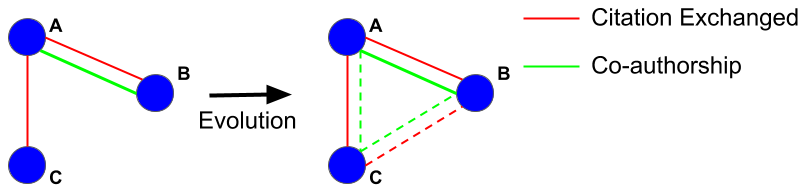
\includegraphics[scale = 0.28]{plots/goals}
	
	\captionsetup{singlelinecheck=false, justification=raggedright,  labelsep=space}
	\caption{Possibile events as the citation and co-authorship networks evolve. Dotted lines indicate Possibility of event occuring at later time given the existing events(solid) at previous time.}
	\label{f1}
\end{figure}

Fig.\ref{f1} summarizes the possible events in the evolution of collaboration networks. 

In the following sections we explain the construction of Distance and Citation matrices followed by our results and empirical calculations. We conclude with our discussion and future work.

\section{Methods}

\subsection{Data Matrices}

We construct cumulative bipartite graphs of (top nodes)papers and (bottom nodes)authors from 1970-2013 for Indian publications in APS journals. We also construct two sets of citation graphs i) cumulative including all citations and ii)non-cumulative with citations only between Indians, for each year. We then remove naming dis-ambiguity and check manually for possible repetitions in names. After pre-processing the number of unique authors who had Indian affiliation were 8084. Each node(author) in the co-authorship network is assigned a unique ID and the nodes are ordered alphabetically which is kept consistent for all calculations

Matrices of size($N\times N$) where $N = 8084$ defined below, capturing distance between two pairs(ij) of authors and citations exchanged between them were constructed for every time period.

$D_{ij}(t) = 	\begin{cases} d_{ij} ,$ if ij have a path$ \\
                         			0 $ otherwise$
           		\end{cases}$ \\

$D_{ij}(t)$ captures the distance between each pair of nodes in that network. It is to be noted that $D_{ij} = 0$ can also mean that the nodes do not exist in the network at that time.   

$C(t) = 	\begin{cases} 	C^{ij}_{in} ,$ number of times j cites i $ \\
                           C^{ji}_{out} ,$ number of times i cites j $
           	\end{cases}$\\
 
$C(t)$ stores the citations exchanged between papers written by i and j for the given time t. The citations recorded are cumulative. The above citation and distance matrices store the history of interactions between all possible author  $\binom{N}{2}$ where $N = 8084$ from 1970-2013. We use these matrices for all our calculations in the paper.

For tracing the history of co-authorship events fig\ref{f4}, we extract the distance 1 collaborations at the end of data (edges in 2013 co-authorship graph). We then trace the presence of edge between i and j (contributing authors) in reverse. The time when the edge 1st appears is marked $T_c$. Then we check for the presence of i and j in the network before $T_c$ and stop at time $T_0$ when both i and j appear together in the network. The number of citations exchanged by pairs at every time before and after collaboration are recorded. The obtained time series is shifted on the axis to 0 so that we can compare the citation exchanged before and after first collaboration.

The above is done for $\approx 44000$ pairs. Out of these we remove the pairs that had $T_0 = T_c$. The remaining are author pairs who took at least 1 year to collaborate after appearing together in the network($\approx 13000$).  We do the same for pairs that have distance d = 2 and higher in the end and compare with d=1 pairs. 

\subsection{Calculations}

\subsubsection{Cite but do not co-author:} 
For all pairs in Citation matrix at time t $C(t)$, we count the number of pairs $N^C$ with $C(t)_{ij} + C(t)_{ji} != 0$. Among the pairs $N^C$ we count pairs $N^C_{(d!=1)}$ that have $d_{ij} != 1$ and $N^C_{(d=0)}$ $d_{ij} = 0$ given that the network had $N(t)$ nodes at time t.

With $\binom{N(t)}{2}$ possible pairs we can calculate respective fractions 

\subsubsection{Co-author but do not cite:}
For all pairs in Distance matrix (considering only the upper diagonal) at time t $D(t)$ we count pairs $N^D$ with  $D_{ij} = 1$. Among the pairs $N^D$ we count pairs $N^D_{(C_{ij} + C_{ji}=0)}$
\begin{figure}
	\centering
	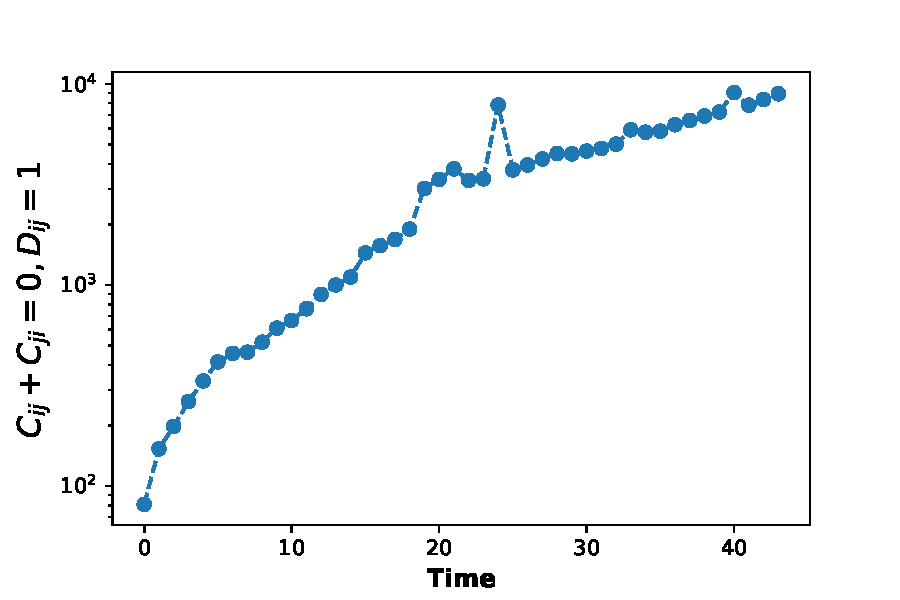
\includegraphics[scale = 0.45]{plots/d1_zcit}
	
	\captionsetup{singlelinecheck=false, justification=raggedright,  labelsep=space}
	\caption{Number of author pairs that co-author but do not cite each other.}
	\label{f2}
\end{figure}

\subsubsection{Reciprocity:}
For every author $i$ in the Citation matrix $C(t)$ we define $N_i$ number of authors that cite $i$ and $n_i$ as number of authors whom $i$ cites. Then reciprocity $r_i$ of the author $i$ is defined as $\frac{n_i}{N_i}$. 


\subsubsection{Probability that pairs Co-author given they exchange non-zero citation in the past:}
We define $P(C)$ as probability that they cite each other before collaborating in  $t$ and $P_{n}(c)$ as probability that the pair have cited each $n$ years before collaboration in $t$. 
There fore we have:
\begin{equation}
P(C) = P_{1}(c) + P_{2}(c) + \dots + P_{t-T_0}(c) 
\end{equation}
$T_0$ is time of first co appearance. Let $P(D=1)$ be probability of co-authoring then we have:
\begin{equation}
P(D=1|C) = \frac{P(C|D=1).P(D=1)}{P(C)}
\end{equation}

\subsubsection{Change in average network distance between pairs VS number of citations per pair over time:}
For every Distance matrix $D(t)$ at time t, we measure the distribution of network distances as in fig\ref{f2}. The value of the peak $d^m_{ij}(t)$ for every time, the longest path value $d^l_{ij}(t)$ and the $\bar{d}_{ij}(t)$ at every time step are then plotted against the average number of citations exchanged per pair $\bar{c}$ at time step t.
\begin{equation}
\bar{c} = \frac{\sum_{p_{ij}=1}^{N} C_{p_{ij}} + C_{p_{ji}}}{N} 
\end{equation}
$p_{ij}$ is pair that have non zero mutual citations, $C_{p_{ij}} + C_{p_{ji}}$ is total citations exchanged between $p_{ij}$ and N is number of such pairs.
\section{Results}

\begin{figure*}[htbp]  
	\centering
		
	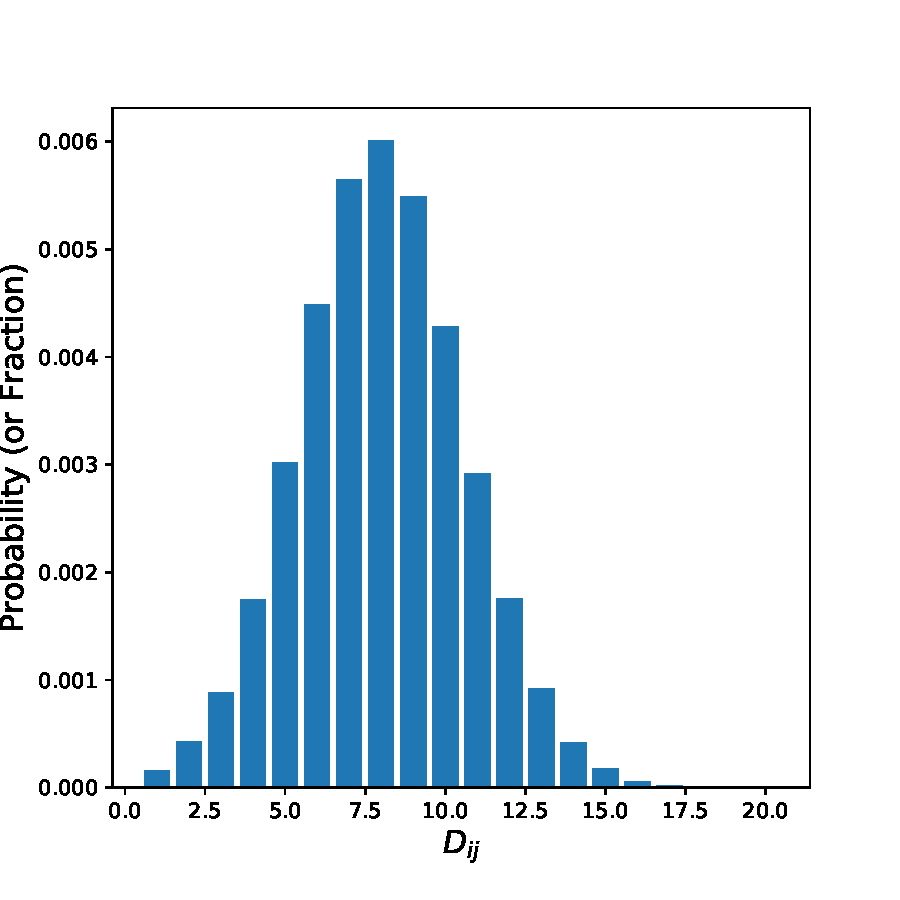
\includegraphics[scale = 0.33]{plots/Dij_dist_hist_1990}
	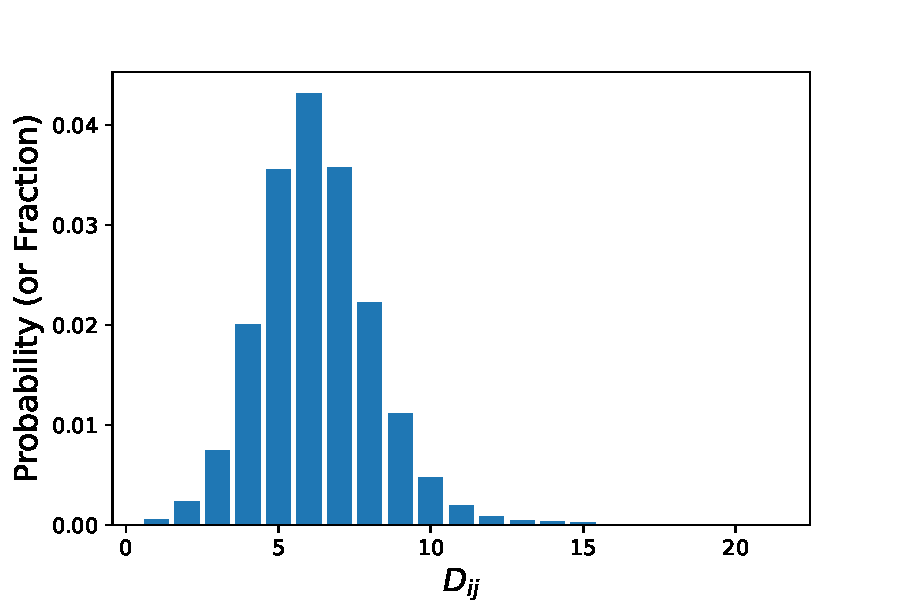
\includegraphics[scale = 0.33]{plots/Dij_dist_hist_2000}
	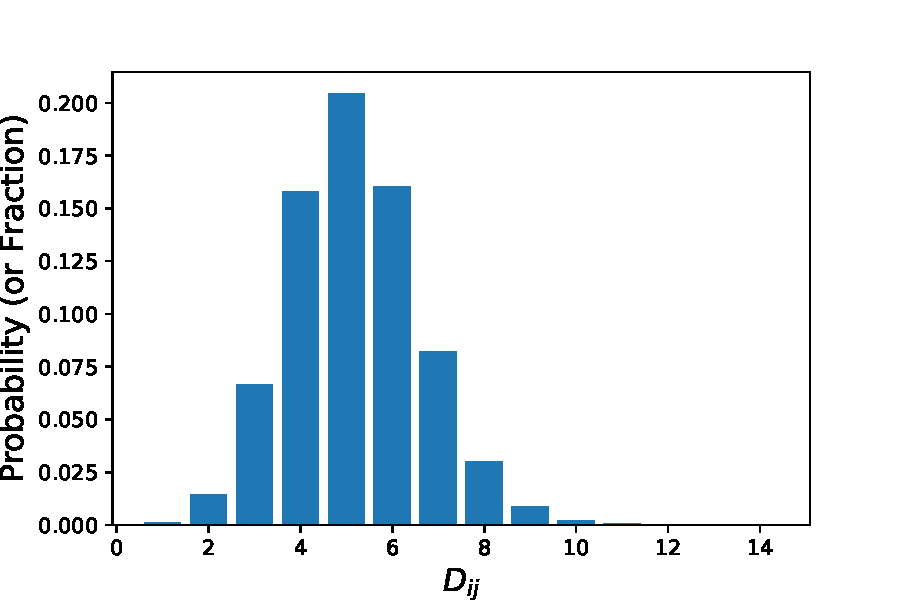
\includegraphics[scale = 0.33]{plots/Dij_dist_hist_2013}
	
  \captionsetup{singlelinecheck=false, justification=raggedright,  labelsep=space}
  \caption{The distribution ratios of distanes $d_{ij}$ between pairs for the years 1990,2000 and 2013 (left to right)}
  \label{f3}
\end{figure*}
In Fig.\ref{f3} the spread in distance matrices(top panel) is proportional to the network size. Distribution of distances in the network as it  evolves shows the increased connectivity between authors at different distances. Pairs that have no existing path have been excluded in the above graphs. The d value for the peak of the distribution(5 in the final graph) and the spread from the mean(variance) decreases as the network evolves with time. The decreasing values for the peak and variance are due to the increase in connectivity of the network. 

{\color{blue}We should compare this with existing analytical function for distances in a network(probably Newman has some review over this) and see if we can explain the pattern in a much better way.}

\begin{figure}
	\centering
	
	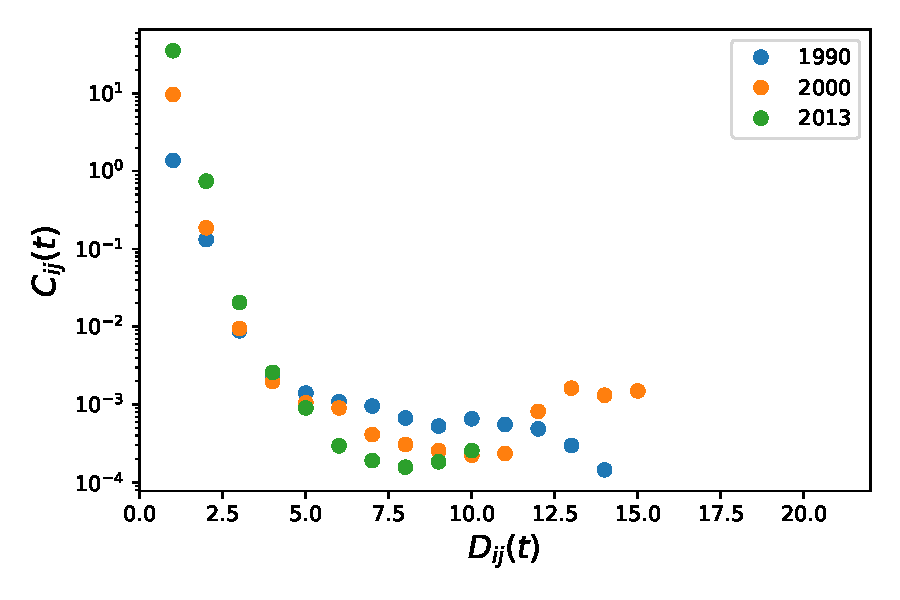
\includegraphics[scale = 0.49]{plots/fig1}
	
\captionsetup{singlelinecheck=false, justification=raggedright,  labelsep=space}
\caption{Total number of citations between pairs of authors VS distance D between pairs in the co-authorship network(for all years till 2013)}
   \label{f4}
\end{figure}

\begin{figure*}
	\centering

	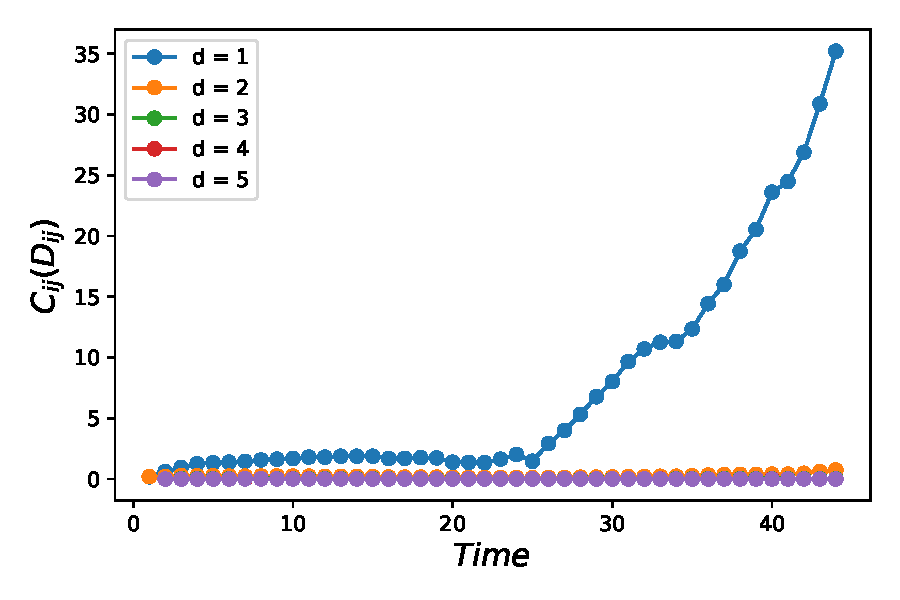
\includegraphics[scale = 0.49]{plots/fig2}
	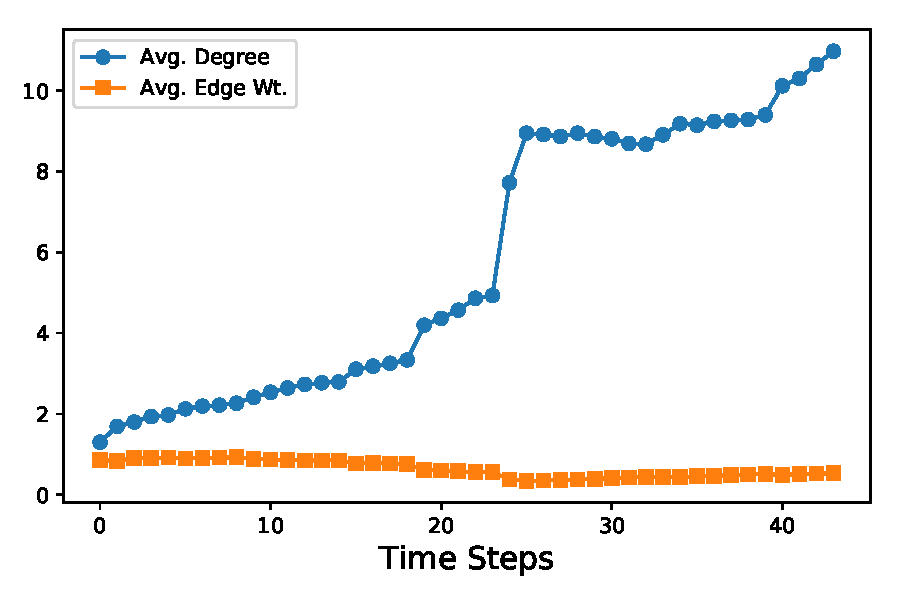
\includegraphics[scale = 0.49]{plots/fig3}
	\captionsetup{singlelinecheck=false, justification=raggedright,  labelsep=space}
	
	\caption{Change in the number of citations exchanged between pair ij at distance D with time}
	\label{f4a}
\end{figure*}

The number of citations exchanged by pairs ij of authors at distance d apart in the co-authorship network for a time t falls almost exponentially as in Fig\ref{f4}. We ignore the citation exchanged between pairs that have no path in between.(Reason of doing this? Maybe because we are only interested in seeing the change in citations with your near or distant collaborators).

Another way to look at the same is to measure the rate of change of citations exchanged between ij pairs at a distance d for the time series data Fig\ref{f4a}. We notice that for direct collaborations(co-authorship events) the rate of citations exchanged increase with time with a sudden transition post 1995 which is also true for average degree of nodes as shown in figure. However the growth rate falls rapidly for distance 2 between pairs and is almost zero for distance 3 and higher. {\color{blue}This means that the citations exchange between ij pairs far in the co-authorship network could be considered as random.}

The change in the strength of collaboration between two authors i and j can be seen in fig\ref{f5}. Here the strength of collaboration is indicated by the total citations exchanged by i and j in that time period through their papers. This includes cases where i and j cite there previously written paper. For our case this adds to the strength. 

{\color{red}Literature review suggests that there is a threshold time for every paper to be discovered for citation hence it would be very uncommon for authors to cite papers published in the same year of their publication unless they know they know the authors or are working together. for ex. I would know more about my colleagues papers}



\begin{figure*}[htbp]  
	\centering
	
	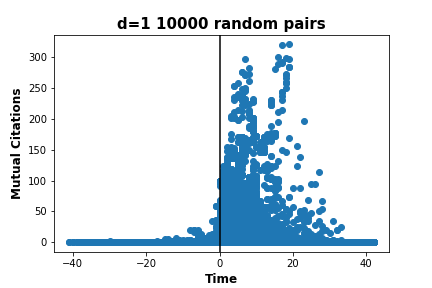
\includegraphics[scale = 0.49]{plots/d1}
	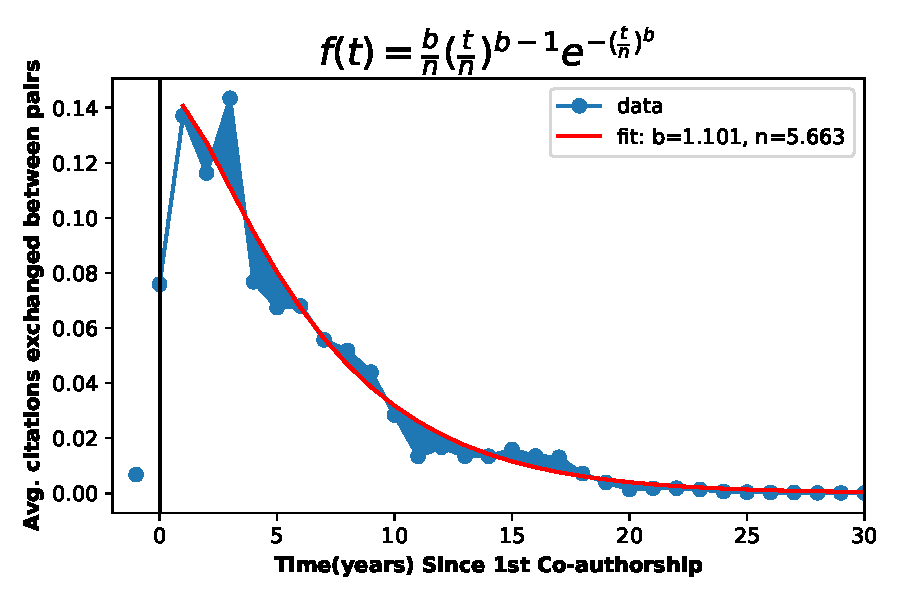
\includegraphics[scale = 0.49]{plots/aging_in_colab}
		
\captionsetup{singlelinecheck=false, justification=raggedright,  labelsep=space}
\caption{Distribution of citations exchanged before and after Time of first co-authorship event between authors. The sudden peak and rise is an interesting observation specially the decay part.}
   \label{f5}
\end{figure*}

\begin{figure*}[htbp]  
	\centering
	
	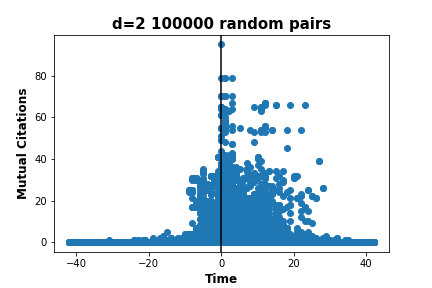
\includegraphics[scale = 0.49]{plots/d2}
	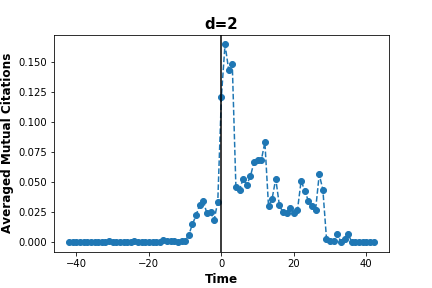
\includegraphics[scale = 0.49]{plots/d2_avg}
	
	\captionsetup{singlelinecheck=false, justification=raggedright,  labelsep=space}
	\caption{Distribution of citations exchanged before and after Time of first co-authorship event between authors. The sudden peak and rise is an interesting observation specially the decay part.}
	\label{f6}
\end{figure*}

It is observed that the citations exchanged peak after 1st collaboration and then fall. Interestingly the peak for this distribution is within 4 years of $T_c$. The mean active period for Indians is around 4.5 years (from our previous study). The decay observed fits well with the Weinbull distribution defined as :

\begin{equation}
 f(t) = \frac{b}{n}(\frac{t}{n})^{b-1} e^{-(\frac{t}{n})^b}
\end{equation}

{\color{blue}This function as discussed in the paper in PNAS(cite the PNAS aging paper) defines the change in probability of a paper receiving a citation after t years of publication.}

In our case it represents the decay in strength of collaboration. We need to explain the significance of parameters b and n in distribution. The observed decay in strength of collaboration can be an implicit cause due the aging function for probability of a paper receiving citation as proposed in the paper(PNAS). 

\section{Conclusion}

\section{References}

\end{document}